\documentclass[11pt]{article}
\usepackage[a4paper,margin=2cm]{geometry}
\usepackage{amsmath}
\usepackage{graphicx}
\usepackage{enumitem}
\usepackage{booktabs}
\usepackage{array}
\usepackage{xcolor}
\usepackage{parskip}
\setlist{itemsep=3pt, topsep=3pt}
\newcommand{\menu}[1]{\textbf{#1}}

\begin{document}

{\LARGE\bfseries MQTT test: NodeMCU $\rightarrow$ broker $\rightarrow$ laptop}\\[4pt]
The NodeMCU publishes its own stats every 2 seconds to topic \texttt{test/01}; a Python script on the laptop receives and prints them.

\section*{Files in this folder}
\begin{tabular}{@{}>{\ttfamily}l l@{}}
nodemcu\_mqtt\_pub/nodemcu\_mqtt\_pub.ino & Publisher. Arduino sketch (C++) for the NodeMCU. \\
sub.py & Subscriber. Python script for the laptop. \\
\end{tabular}

\section*{How it fits together}
\begin{center}
\texttt{NodeMCU (publisher)} $\xrightarrow{\ \mbox{\small Wi-Fi, MQTT}\ }$
\texttt{Broker (Mosquitto)} $\xrightarrow{\ \mbox{\small MQTT}\ }$
\texttt{sub.py (subscriber)}
\end{center}
The broker is the ``post office'': the NodeMCU posts messages to topic \texttt{test/01}, and every program subscribed to \texttt{test/01} gets a copy.
The sender (C++) and the receiver (Python) don't need the same language: they both speak the MQTT protocol.

\section*{Choose your setup first}
The sketch has a \textbf{broker block}: keep \textbf{exactly one} \texttt{BROKER} line uncommented.
\texttt{sub.py} takes the broker as an argument instead (no editing), and must point to the \textbf{same broker} as the sketch.

\begin{tabular}{@{}>{\raggedright}p{3.6cm} >{\raggedright}p{6.2cm} >{\raggedright\arraybackslash}p{6.4cm}@{}}
\toprule
 & \textbf{Option A: broker on your laptop} (default) & \textbf{Option B: public broker} \\
\midrule
In the sketch & \texttt{BROKER = "<laptop IP>"} & \texttt{BROKER = "broker.hivemq.com"} \\
Run \texttt{sub.py} & \texttt{python sub.py} (= localhost) & \texttt{python sub.py broker.hivemq.com} \\
Needs internet? & No. Traffic stays on the local Wi-Fi. & Yes. \\
Works on college Wi-Fi? & Yes (tested) & \textbf{No}: the college network blocks MQTT to the internet \\
Works on phone hotspot? & Yes & Yes \\
Needs Mosquitto installed? & Yes, on the laptop & No \\
Private? & Yes & No: anyone can read topic \texttt{test/01} \\
\bottomrule
\end{tabular}

\vspace{6pt}
\textbf{What about the proxy?} The proxy (host \texttt{172.31.2.3}, port \texttt{8080}) is only for reaching the internet, and it
\textbf{cannot carry MQTT}: it only allows HTTPS-style connections on port 443, and the MQTT ports are refused (tested).
So there are no proxy lines in the code:
\begin{itemize}
\item Option A never needs the proxy (local traffic).
\item Option B needs a \textbf{phone hotspot with the laptop's proxy turned OFF}.
\item The proxy is only needed in \textbf{Arduino IDE} on the college network, to download the library in step 1
(\menu{File $\rightarrow$ Preferences $\rightarrow$ Network $\rightarrow$ Manual proxy}, host \texttt{172.31.2.3}, port \texttt{8080}, no username/password).
\end{itemize}

\newpage
\section*{Step 1: Install the MQTT library in Arduino (once)}
\begin{enumerate}
\item Arduino IDE $\rightarrow$ \menu{Tools $\rightarrow$ Manage Libraries\dots}
\item Search \textbf{PubSubClient}.
\item Install \textbf{``PubSubClient by Nick O'Leary''}.
\end{enumerate}
On the laptop, Python needs \texttt{paho-mqtt}: \texttt{pip install paho-mqtt} (once).

\section*{Step 2: Open and edit the sketch}
\begin{enumerate}
\item \menu{File $\rightarrow$ Open} $\rightarrow$ \texttt{nodemcu\_mqtt\_pub/nodemcu\_mqtt\_pub.ino}
\item Edit the lines at the top:
\begin{verbatim}
const char* WIFI_SSID = "IIITA";          // Wi-Fi name
const char* WIFI_PASS = "";               // Wi-Fi password ("" if none)
const char* TOPIC     = "test/01";
const char* BROKER = "172.29.0.43";       // OPTION A: laptop IP
// const char* BROKER = "broker.hivemq.com"; // OPTION B: public
\end{verbatim}
\item \textbf{Option A:} find the laptop's IP with \texttt{ipconfig} (Windows) $\rightarrow$ \textit{Wireless LAN adapter Wi-Fi} $\rightarrow$ \textit{IPv4 Address}.
It can change from day to day, so check it again if the NodeMCU suddenly cannot connect.
\item The Wi-Fi must be \textbf{2.4 GHz} (ESP8266 cannot see 5 GHz). On a phone hotspot choose the 2.4 GHz band / ``Maximize Compatibility''.
\end{enumerate}

\section*{Step 3: Upload}
\begin{enumerate}
\item Plug in the NodeMCU, select board \textbf{NodeMCU 1.0 (ESP-12E Module)} and its \textbf{COM port}.
\item Close the Serial Monitor if open, then click \menu{Upload}.
\end{enumerate}

\section*{Step 4: Watch the NodeMCU}
\menu{Tools $\rightarrow$ Serial Monitor}, \textbf{9600 baud}, press \textbf{RST}. Good output:
\begin{verbatim}
Connecting to Wi-Fi 'IIITA'.....
Wi-Fi OK, my IP: 172.29.x.x
Connecting to MQTT broker 172.29.0.43 ... OK
Publishing to topic: test/01
sent  {"uptime_s":3,"rssi_dbm":-55,"free_heap":50112,"a0":4}
\end{verbatim}

\section*{Step 5: Receive on the laptop}
Open PowerShell in this folder and run:
\begin{verbatim}
cd C:\path\to\mqtt_test
python sub.py                    # broker = localhost (this laptop)
python sub.py 172.29.1.135       # broker = another machine, e.g. the Pi
python sub.py broker.hivemq.com  # public broker (hotspot only)
\end{verbatim}
Use the one that matches \texttt{BROKER} in the sketch. Every 2 seconds:
\begin{verbatim}
13:04:13  test/01  {"uptime_s":63,"rssi_dbm":-89,"free_heap":50112,"a0":4}
\end{verbatim}
Stop with \textbf{Ctrl+C}.

\newpage
\section*{What the values mean}
\begin{tabular}{@{}>{\ttfamily}l >{\raggedright\arraybackslash}p{13cm}@{}}
\toprule
\textrm{\textbf{Field}} & \textbf{Meaning} \\
\midrule
uptime\_s & Seconds since the NodeMCU last started. Goes up by 2 each message. Drops back to 0 if the board restarts. \\
rssi\_dbm & Wi-Fi signal strength in dBm. Always negative; \textbf{closer to 0 = stronger}.
About $-50$ excellent, $-70$ good, $-85$ weak, $-90$ barely working. Move the board closer to the router/hotspot and watch it rise. \\
free\_heap & \textbf{Free RAM in bytes.} The ESP8266 has about 80 KB of RAM; around 50{,}000 bytes free is normal for this sketch.
If it stays constant (it should), there is no memory leak. If it slowly falls, the program is leaking memory. \\
a0 & Reading of the analog pin A0, from 0 to 1023 (0 V to about 3.3 V). Nothing is connected, so it shows small random noise (about 0--10).
Touch the pin with a finger and it jumps. A real analog sensor (e.g.\ a light sensor) would go here. \\
\bottomrule
\end{tabular}

\vspace{6pt}
These are placeholder ``sensor'' values, because the ESP8266 has \textbf{no built-in temperature sensor}. Later a DHT22 replaces them with real temperature and humidity.

\section*{Troubleshooting}
\begin{tabular}{@{}>{\raggedright}p{5.6cm} >{\raggedright\arraybackslash}p{10.6cm}@{}}
\toprule
\textbf{Symptom (Serial Monitor)} & \textbf{Cause / fix} \\
\midrule
Stuck on \texttt{Connecting to Wi-Fi.....} & Wrong name/password, network is 5 GHz, or it needs a browser/username login (ESP8266 can't do that). Use a phone hotspot. \\
\texttt{failed (state -2)} repeating & Can't reach the broker. Option A: wrong laptop IP, Mosquitto not running, or the network blocks device-to-device traffic. Option B: you are on the college network; use a hotspot. \\
Gibberish & Serial Monitor baud must be 9600 (same as \texttt{Serial.begin(9600)} in the sketch). \\
\texttt{sub.py} connects but prints nothing & Different broker or topic than the sketch. Both files must use the same option and \texttt{test/01}. \\
\texttt{sub.py}: \texttt{ConnectionRefusedError} & Option A: Mosquitto is not running on the laptop. \\
\bottomrule
\end{tabular}

\vspace{6pt}
\textbf{Mosquitto on Windows (option A), one-time setup:} in \texttt{C:\textbackslash Program Files\textbackslash mosquitto\textbackslash mosquitto.conf} add
\texttt{listener 1883 0.0.0.0} and \texttt{allow\_anonymous true}, restart the Mosquitto service, and allow TCP port 1883 in Windows Firewall.
Without this, Mosquitto only accepts connections from the laptop itself.

\newpage
\section*{Result (tested)}
Option A on the college Wi-Fi. Left: NodeMCU sketch and its Serial Monitor (\texttt{sent \{...\}}).
Right: \texttt{python sub.py} on the laptop receiving the same messages on \texttt{test/01} every 2 seconds.

\vspace{6pt}
\begin{center}
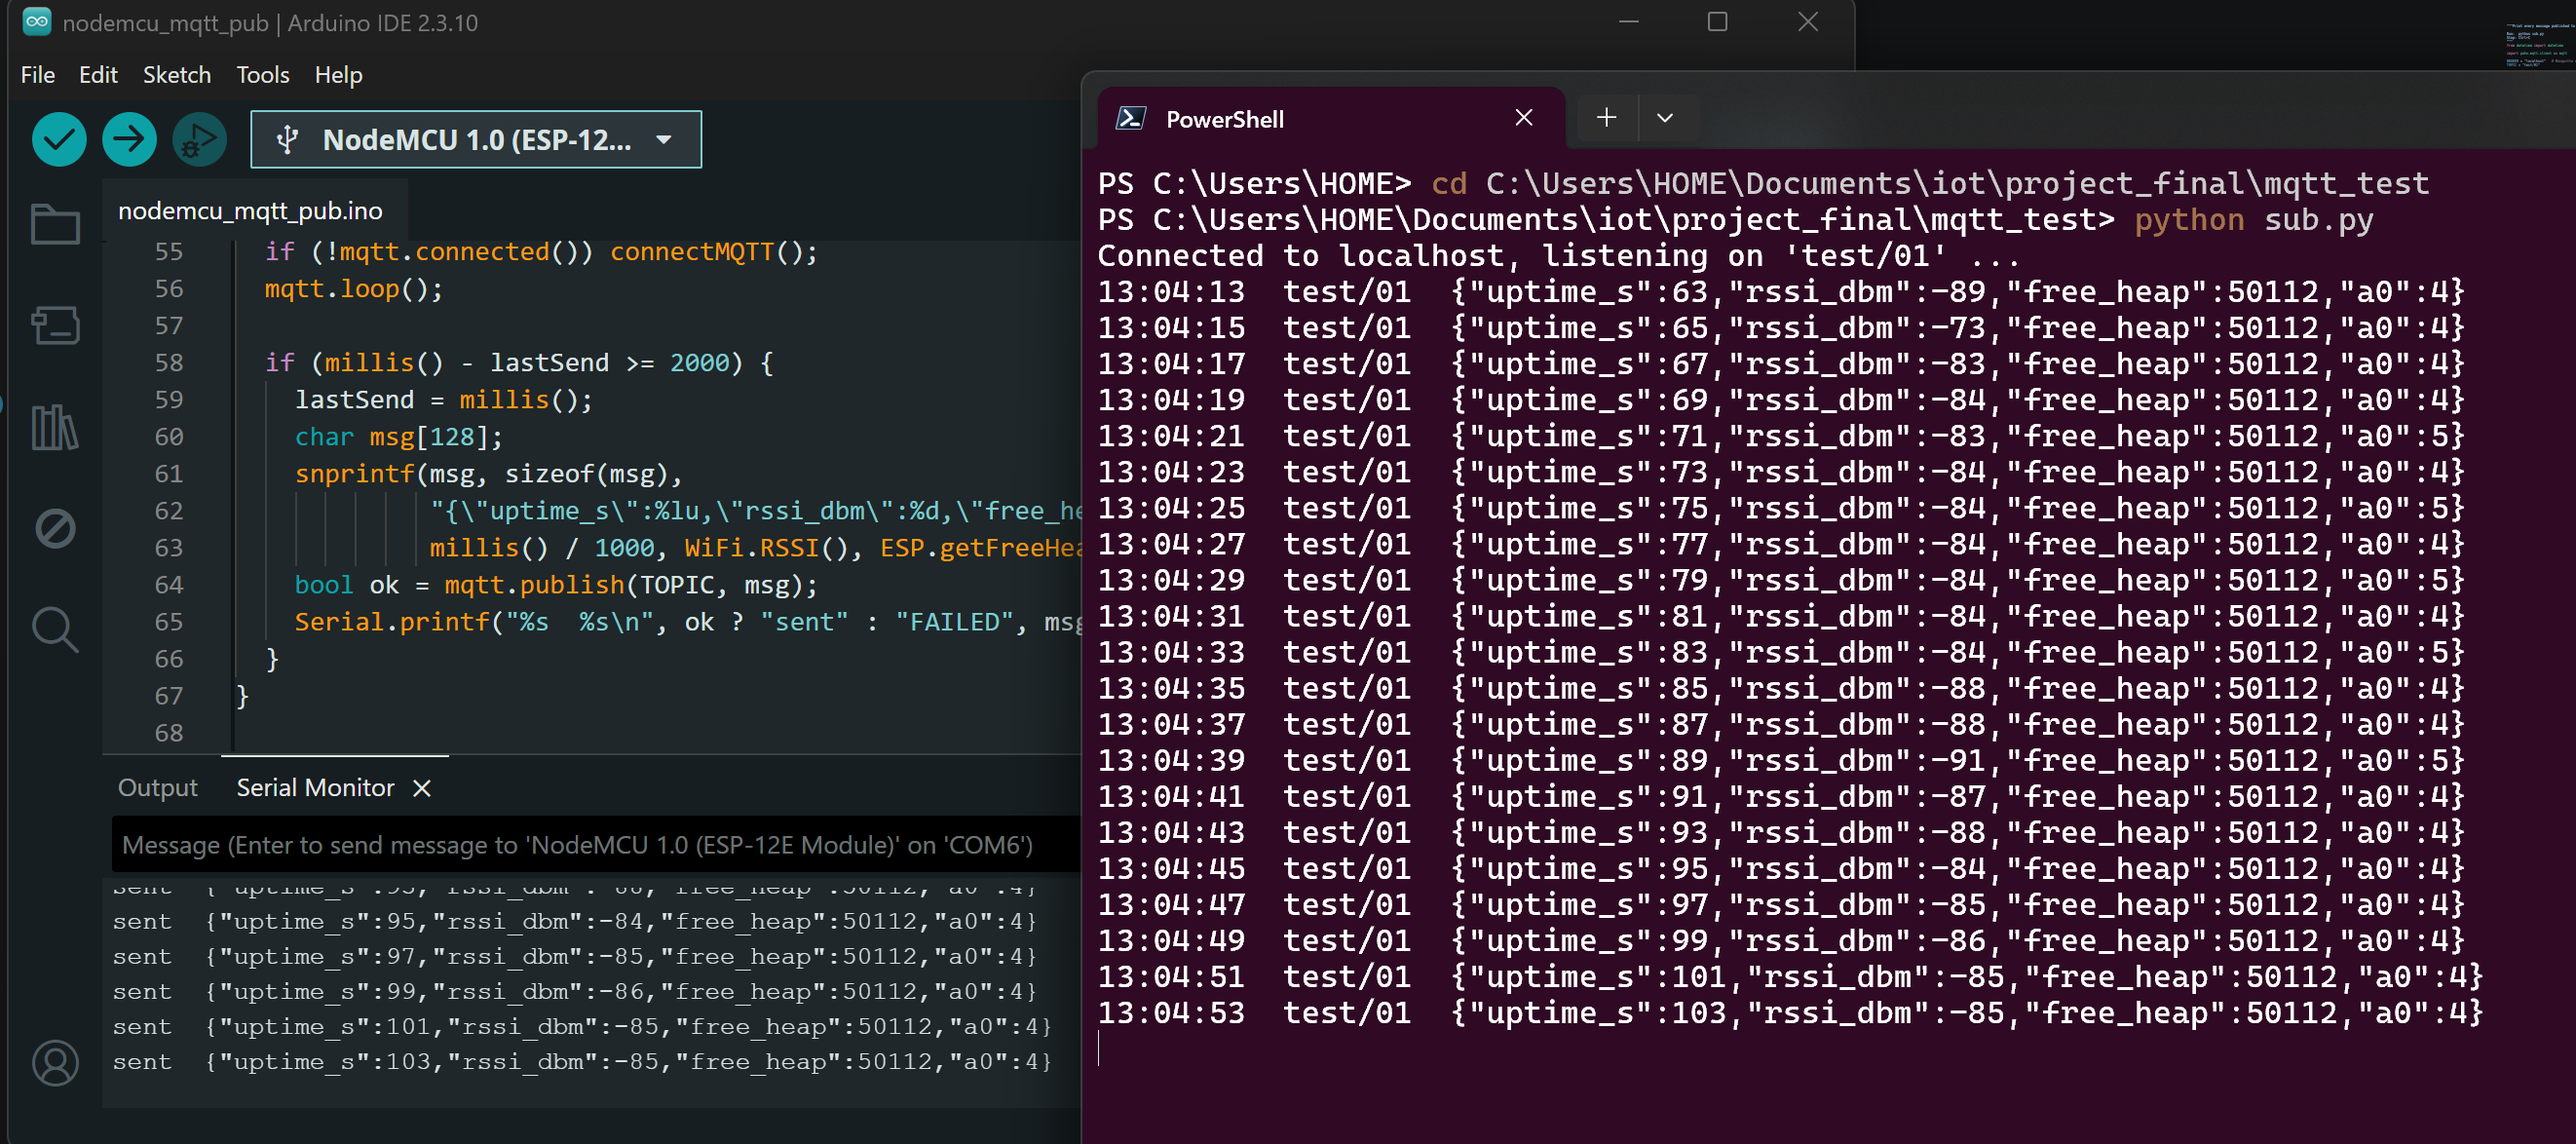
\includegraphics[width=\textwidth]{img/mqtt_result.png}
\end{center}

\end{document}
